\section{TinyDAS}

This section introduces TinyDAS, a Python framework specifically made for scalable model training on \acrshort{das} data to detect anomalies within \acrshort{das} data. 

\subsection{Tools}

Tinygrad is a neural network framework created by George Hotz in October 2020 \cite{tinygrad2020}. It is based on Andrej Karpathys' library \texttt{Micrograd} \cite{micrograd}, which aims to strip neural network frameworks down to its core. Tinygrad was introduced as an alternative to other popular frameworks such as Pytorch \cite{paszke2019pytorch} and TensorFlow \cite{abadi2016tensorflow}. The main goal is to \textquote{Build an equal performance stack to Pytorch on NVIDIA and AMD} \footnote{As stated in a conversation between George Hotz and Lex Fridman \cite{LexClipsYouTube2023}}. Unlike its alternatives, Tinygrad strives towards being hardware agnostic, where writing codes for different accelerators should be as similar as possible. For organizations, such as \acrshort{cgf} with limited hardware resources, this allows for an overall cheaper entry into scalable \acrshort{ml}, without sacrificing performance. \\

All operations in Tinygrad are lazy \cite{tinygrad}. This means that a binary operation on two tensors, such as $a+b$, is not computed until the operation is realized. Additionally, \texttt{Tinygrad} strives for a more functional design pattern with a limited amount of classes. Furthermore, \texttt{Tinygrad} has a built-in \acrfull{jit} compiler, in which a kernel can be replayed, allowing for faster operations such as a \texttt{train} function. For anomaly detection, we utilize several popular Python packages such as \texttt{numpy}, \texttt{scikit-learn} and \texttt{seaborn} for evaluation metrics, and \texttt{matplotlib} for visualization and plots. A full list of packages used can be found in 
appendix \ref{app:tinypacks}.


\subsection{Overview}
\label{meth:tinyoverview}

TinyDAS consists of two parts. The first part handles model construction and training, while the latter deals with anomaly detection of \acrshort{das} data. An overview of how TinyDAS works is shown in Figure \ref{fig:dataflow}. The following list outlines the fundamental principles and criteria used to design and evaluate the framework:

\clearpage

\begin{enumerate}
    \item \textit{Support} for memory-efficient training techniques, specifically half-precision
    \item \textit{Scalability} from single-core systems to multi-node clusters
    \item \textit{Hardware agnostic} to ensure wide usability
    \item \textit{Modular architecture}, easily extendable with new models
    \item \textit{Separation of core logic} from data workflow for improved maintainability
    \item \textit{Collection} of different algorithms for anomaly detection
    \item \textit{Future potential} for online anomaly detection in a live environment
    \item \textit{Model-agnostic} approach to anomaly detection for broader applicability
\end{enumerate}

\begin{figure}[!h]
    \centering
    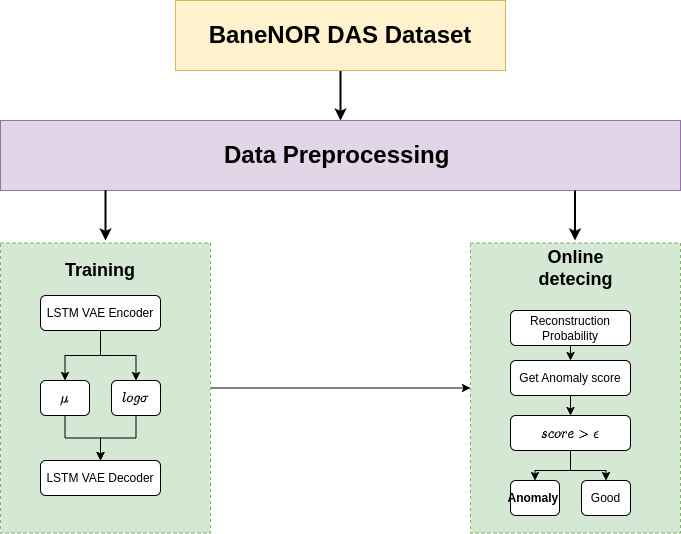
\includegraphics[scale=0.5]{figures/methodflow.png}
    \caption{Overview of TinyDAS. It takes a \acrshort{das} dataset, preprocess it, and depending on task, either trains an autoencoder or uses an already trained model to detect anomalies within a dataset.}
    \label{fig:dataflow}
\end{figure}

\subsection{Core Functionality}

Due to Tinygrad's relatively simple framework, we can implement custom components intended to be reusable and modular for our specific use case.

\subsubsection{Datasets and Dataloaders}

The \texttt{Dataset} and \texttt{DataLoader} classes support loading \acrshort{hdf5} in parallel batches, with support for data normalization and type casting. The former handles information about the dataset to be trained on and logic for loading a single file from a \acrshort{hdf5} file or whatever other format might be sent later. The latter handles parallel batches loading $n$ samples into the model.

\subsubsection{Autoencoder Base Class}

\lstinline{BaseAE} is the base model class from which all models are inherited. When training a model, the \lstinline{criterion} method is the main method to call. It runs the \lstinline{__call__} method and applies the loss function of choice.  We define the class as follows:

\lstinputlisting[language=Python, label={lst:baseae}, caption=Base Autoencoder class]{code/baseae.py}

\acrshort{vae} models returns both reconstructed output, as well as the $\mu$ and $\sigma$ layers to calculate the \acrshort{elbo} loss. To make the \lstinline{__call__} method support both regular and variational autoencoders, we return a tuple.
In addition to the methods shown in Code Listing \ref{lst:baseae}, this class includes code for saving and loading, as well as different weight initialization methods such as \textit{He}- and \textit{Xavier} initialization \cite{kumar2017weight}. Proper weight initialization is important to avoid vanishing or exploding gradients, as discussed in \cite{narkhede2022review}. 

\subsubsection{Trainer}

The Trainer class serves as the core component of our program. As demonstrated in Code Listing \ref{fig:lstmcell}, it integrates a model, dataloader, and optimizer to execute the training process. Additionally, it handles early stopping, stores the history of losses, and saves the best model for further use. The \texttt{Trainer} class is shown in code listing \ref{code:trainer} in the appendix. Note that the \lstinline{@TinyJit} decorator enables kernel replays on subsequent calls, speeding up training and validation. 


One of the more important aspects of this class is the \texttt{train} function, which leverages Tinygrad's \acrshort{jit} compiler to replay the kernel for each iteration, resulting in faster training times. Both the early stopping mechanism and the learning rate scheduler are designed to use validation loss by default. We continuously check the performance of each epoch and store the model parameters for each epoch, which later can be loaded, enabling transfer learning. The full trainer class can be seen in Code Listing \ref{code:trainer} in the appendix.


\subsection{General Usage}

\subsubsection{Training}

TinyDAS supports training and prediction with half-precision to optimize computational efficiency. This feature, which can be activated through configuration files, converts all weights and biases in the model to half-precision floating-point format, effectively reducing memory requirements for training. In the same way that \texttt{Judas} is designed, we want \texttt{TinyDAS} to be modular and easy to use. We've designed components in a way that is familiar to that of Pytorch \cite{paszke2019pytorch}, but without having to specify hardware or do many configurations to enable either half-precision training/inference or data-parallel training. Models can be trained using the following script:

\lstinputlisting[caption=Example of how models within \texttt{TinyDAS} can be trained, language=Python]{code/tinydas_main.py}



For example, to initiate training of an autoencoder model using transfer learning on four \acrshort{gpu} devices, one would execute the following command:
\begin{lstlisting}[style=shellcommand, language=bash]
(*@\textcolor{promptcolor}{\$}@*) python main.py -m ae -t train -g 4 -l
\end{lstlisting}

where:
\begin{description}
\item[\texttt{-m ae}] specifies the autoencoder model
\item[\texttt{-t train}] sets the task to training
\item[\texttt{-g 4}] allocates four \acrshort{gpu} devices
\item[\texttt{-l}] enables transfer learning
\end{description}

This approach allows for flexible training of all TinyDAS models, accommodating various hardware configurations and leveraging pre-trained models through transfer learning. The model parameters are stored in the \texttt{safetensors} file format \cite{safetensors}.

\subsubsection{Hyperparameters and configurations}

Hyperparameters for the different models are stored in separate YAML files with the same name as the model. An example of a hyperparameter configuration can be found in appendix \ref{app:hyper}.


\subsubsection{Anomaly Detection}

TODO: Speak about this program can be called to run in anomaly mode!!

 
After training the models on normal signal data, we move on to the anomaly detection section of our program. As mentioned in Section \ref{back:anomdet}, first decide which types of anomalies are to be found. We decided to first of all split the files into smaller files of \qty{5}{\si{\second}} files, partially to facilitate faster inference of our model. We decided to look at the whole array instead of finding segments. We will calculate precisions, recalls, and f1scores to find a threshold for reconstruction loss of our data and determine whether or not the data is anomalous. A function for finding this threshold is presented in Code Listing \ref{code:th}.  \\

\lstinputlisting[language=Python, caption=Code for finding the best threshold, label={code:th}]{code/bestth.py}

By finding the optimal threshold, we can utilize this in an online environment, preprocessing incoming \acrshort{das} data to fit our model and mark the data as anomalous if the reconstructed error is greater than the threshold. 


